\documentclass{beamer}
\usepackage[frenchb]{babel}
\usepackage[utf8]{inputenc}
\usepackage[T1]{fontenc}
\usetheme{Goettingen}

\begin{document}


\title[identification DMRs] 
{Analyse différentielle des régions methylées}
\author{Jakobi Milan}
\institute{TIMC-Imag}
\date[KPT 2004]{Vendredi 15 mars 2019}
\titlegraphic{
\includegraphics[width=0.5\textwidth,height=2cm]{logo_timc.png}}

\frame{\titlepage}

\begin{frame}
\frametitle{Revue de la littérature}
\begin{itemize}
\item Lecture et présentation de trois articles présentant différentes méthodes de créations de gènes d'intérêt pour l'analyse de la méthylation
\item plusieurs approches : Regions of interest, DMRcate...
\end{itemize}
\end{frame}

\begin{frame}
\frametitle{Récupération des donnée}
\begin{itemize}
\item Les données de methylation (BedChip 450k) pour 507 patients atteints de cancer du poumon à petites cellules squameuses
\item les données d'expression pour les mêmes patients
\item Base de données EPIC pour le référencement des sondes
\item Liste de gènes différientiellement exprimés ( Penda) 
\end{itemize}
\end{frame}

\begin{frame}
\frametitle{Premières visualisations}
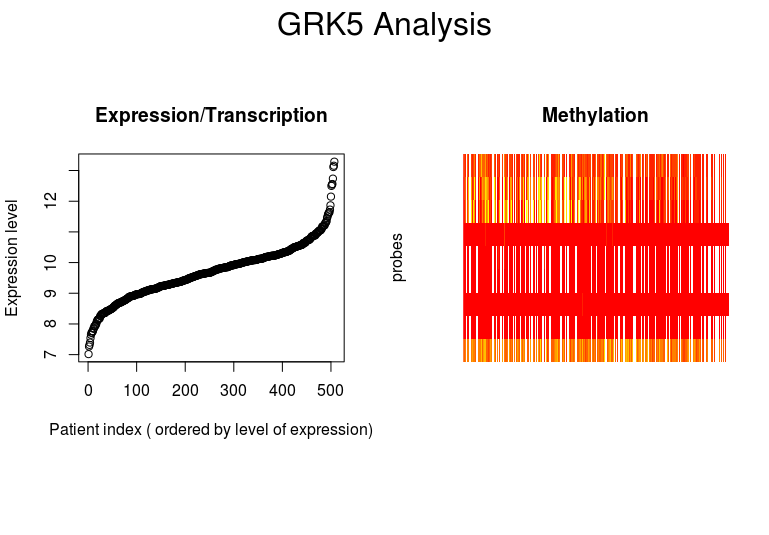
\includegraphics[width=\textwidth]{GRK5_analysis.png}
\end{frame}

\begin{frame}
\frametitle{Premières visualisations}
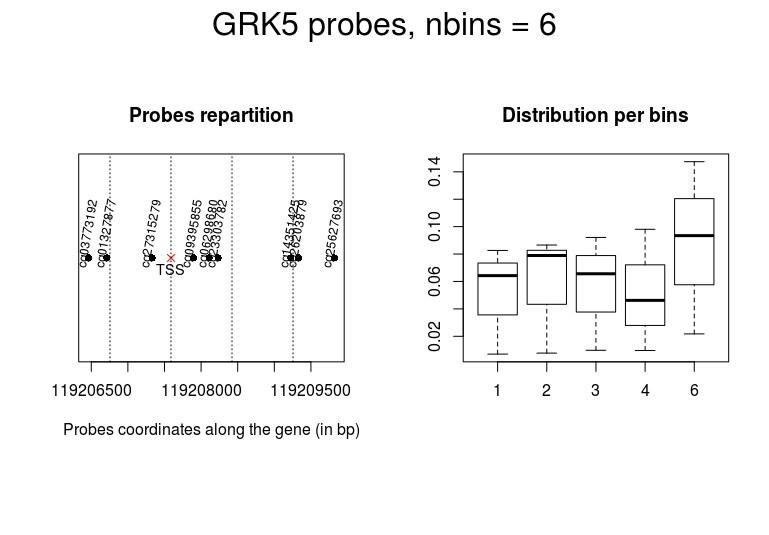
\includegraphics[width=\textwidth]{GRK5_binplot.png}
\end{frame}

\begin{frame}
\begin{itemize}
\item Refaire une visualisation centrée sur le TSS avec des bins à fenêtre fixée (-2500;-1000;-500;TSS;500;1000;2500)
\item En extraire une heatmap ( de la variance/de la moyenne) clusterisée par ces deux variables conjointes.
\item ...
\end{itemize}
\end{frame}








\end{document}